%! Author = gramic
%! Date = 26.03.24

% Preamble
\clearpage
\begin{flushleft}
    \paragraph{Gegebene Parameter und Annahmen}
    Es wird mit fünf Jahren gerechnet.
    Daher werden also die Zeitaufwände der Betriebstasks pro Jahr berechnet und mit fünf multipliziert.
%    Es wurden also folgende Annahmen getroffen resp. folgende Parameter sind gegeben:
    Folgende getroffenen Annahmen und Parameter sind gesetzt:
    \begin{table}[H]

\resizebox{\columnwidth}{!}{%

\begin{tabular}{lrl}
\toprule
Variable & Wert & Beschreibung / Begründung \\ \hdashline
\midrule
Anzahl betrachtete Jahre & 5 & \begin{tabular}[c]{@{}l@{}}\end{tabular} \\ \hdashline
Anzahl Switchovers pro Jahr & 10 & \begin{tabular}[c]{@{}l@{}}Alle zwei Monate wird am KSGR ein Reboot\\der Linux Server für das Patching vorgenommen.\end{tabular} \\ \hdashline
Anzahl Node Recoveries pro Jahr & 5 & \begin{tabular}[c]{@{}l@{}}Mindestens zweimal wird ein Failover Test gefahren.\\Mit drei weiteren Failovers wird gerechnet.\end{tabular} \\ \hdashline
Anzahl Backup Restores pro Jahr & 5 & \begin{tabular}[c]{@{}l@{}}Mindestens vier Restore Tests müssen gefahren werden.\\Mit einem ungeplanten Restore wird gerechnet.\end{tabular} \\ \hdashline
Anzahl Quorum erweiterungen pro Jahr & 1 & \begin{tabular}[c]{@{}l@{}}Es wird mit nur einer Erweiterung pro Jahr gerechnet.\end{tabular} \\ \hdashline
Stundensatz ICT KSGR [CHF] & 120 & \begin{tabular}[c]{@{}l@{}}\end{tabular} \\ \hdashline
\bottomrule
\end{tabular}
}
\caption{Kostenberechnung - Annahmen} \label{dependencis}
\end{table}

    \paragraph{Varianten}
    Patroni wurde in zwei Varianten aufgeteilt.
    Einmal die Vanilla-Version, die manuell aufgesetzt und verwaltet wird.
    Also so wie es bei der Evaluation gemacht wurde.
\end{flushleft}
\begin{flushleft}
    Es gibt allerdings ein \Gls{GitHub}-Repository, welches die ganze Installation in \Gls{Ansible}-Playbooks verpackt hat.
    Der ganze Prozess wurde analysiert und die Aufwände auch für diese Variante geschätzt.
    An der Punkteverteilung ändert sich entsprechend nichts, da die Architektur die gleiche ist, nämlich \texttt{vitabaks/postgresql\_cluster} \cite{HIQVBEPF}.
    Diese Variante wird nachfolgend \texttt{Patroni - postgresql\_cluster} oder vereinfacht nur \texttt{postgresql\_cluster} genannt.
\end{flushleft}
\clearpage
\begin{flushleft}
    \paragraph{Zeitvergleiche}
    Die Zeiten wurden entsprechend den Erfahrungen mit den drei evaluierten Systemen geschätzt.
    Folgende Aufwände wurden gemessen, geschätzt und extrapoliert:
    %\begin{table}[H]
%
%\resizebox{\columnwidth}{!}{%
%
%\begin{tabular}{llrrrr}
%\toprule
%Phase & Subphase & Patroni - vanilla & Patroni - postgresql-cluster & StackGres - Citus & YugabyteDB \\
%\midrule
%\rotatebox{90}{Initialer Aufwand} & Basisinstallation & 5.0 & 6.0 & 4.0 & 5.0 \\
% & Basiskonfiguration & 5.0 & 5.0 & 5.0 & 5.0 \\
% & Backup Konfiguration & 1.0 & 1.0 & 1.0 & 2.0 \\
% & Monitoring Konfiguration & 2.0 & 2.0 & 2.0 & 2.0 \\
%Secuirty Aufwand & private container registry Integration & 0.0 & 0.0 & 1.0 & 1.0 \\
% & PKI Integration & 3.0 & 3.0 & 3.0 & 3.0 \\
%Erweiterungsaufwand & Automatisierung Backup & 1.0 & 1.0 & 4.0 & 4.0 \\
% & Automatisierung Skalierung & 8.0 & 4.0 & 8.0 & 2.0 \\
% & Self-Healing & 8.0 & 4.0 & 16.0 & 0.0 \\
% & Auto-Recovery & 8.0 & 4.0 & 16.0 & 2.0 \\
% & DB Self-Service & 16.0 & 16.0 & 16.0 & 16.0 \\
%Operationsaufwand / 5 Jahre & Switchover & 50.0 & 25.0 & 50.0 & 0.0 \\
% & Node Recovery & 50.0 & 25.0 & 100.0 & 25.0 \\
% & Backup Recovery & 50.0 & 25.0 & 50.0 & 25.0 \\
% & Quorum erweitern & 30.0 & 20.0 & 5.0 & 5.0 \\
% &  & 237.0 & 141.0 & 281.0 & 97.0 \\
%\bottomrule
%\end{tabular}
%}
%\caption{Gemessene und Extrapolierte Aufwände Bsp.} \label{time_investment}
%\end{table}
%\begin{table}[]
%\centering
%\resizebox{\columnwidth}{!}{%
%\begin{tabular}{@{}lllllll@{}}
%\toprule
%Phase                                           & Suphase                                & Patroni - vanilla & Patroni - postgresql-cluster & StackGres - Citus & YugabyteDB & Filter \\ \midrule
%\multirow{4}{*}{Initialer Aufwand}              & Basisinstallation                      & 600               & 720                          & 480               & 600        & 1      \\ \hdashline[0.5pt/5pt]
%                                                & Basiskonfiguration                     & 600               & 600                          & 600               & 600        & 1      \\ \hdashline[0.5pt/5pt]
%                                                & Backup Konfiguration                   & 120               & 120                          & 120               & 240        & 1      \\ \hdashline[0.5pt/5pt]
%                                                & Monitoring Konfiguration               & 240               & 240                          & 240               & 240        & 1      \\ \hdashline[0.5pt/5pt]
%\multirow{2}{*}{Secuirty Aufwand}               & private container registry Integration & 0                 & 0                            & 120               & 120        & 1      \\ \hdashline[0.5pt/5pt]
%                                                & PKI Integration                        & 360               & 360                          & 360               & 360        & 1      \\ \hdashline[0.5pt/5pt]
%\multirow{5}{*}{Erweiterungsaufwand}            & Automatisierung Backup                 & 120               & 120                          & 480               & 480        & 1      \\ \hdashline[0.5pt/5pt]
%                                                & Automatisierung Skalierung             & 960               & 480                          & 960               & 240        & 1      \\ \hdashline[0.5pt/5pt]
%                                                & Self-Healing                           & 960               & 480                          & 1920              & 0          & 1      \\ \hdashline[0.5pt/5pt]
%                                                & Auto-Recovery                          & 960               & 480                          & 1920              & 240        & 1      \\ \hdashline[0.5pt/5pt]
%                                                & DB Self-Service                        & 1920              & 1920                         & 1920              & 1920       & 1      \\ \hdashline[0.5pt/5pt]
%\multirow{4}{*}{Operationsaufwand / Pro Aktion} & Switchover                             & 120               & 60                           & 120               & 0          & 2      \\ \hdashline[0.5pt/5pt]
%                                                & Node Recovery                          & 240               & 120                          & 480               & 120        & 2      \\ \hdashline[0.5pt/5pt]
%                                                & Backup Recovery                        & 240               & 120                          & 240               & 120        & 2      \\ \hdashline[0.5pt/5pt]
%                                                & Quorum erweitern                       & 720               & 480                          & 120               & 120        & 2      \\ \hdashline[0.5pt/5pt]
%\multirow{4}{*}{Operationsaufwand / 5 Jahre}    & Switchover                             & 6000              & 3000                         & 6000              & 0          & 1      \\ \hdashline[0.5pt/5pt]
%                                                & Node Recovery                          & 6000              & 3000                         & 12000             & 3000       & 1      \\ \hdashline[0.5pt/5pt]
%                                                & Backup Recovery                        & 6000              & 3000                         & 6000              & 3000       & 1      \\ \hdashline[0.5pt/5pt]
%                                                & Quorum erweitern                       & 3600              & 2400                         & 600               & 600        & 1      \\ \bottomrule
%\end{tabular}%
%}
%\caption{Gemessene und Extrapolierte Aufwände}
%\label{tab:time_investment}
%\end{table}

\begin{table}[H]
\centering
\resizebox{\columnwidth}{!}{%
\begin{tabular}{@{}llllll@{}}
\toprule
Phase                                           & Subphase                               & Patroni - vanilla & Patroni - postgresql-cluster & StackGres - Citus & YugabyteDB \\ \midrule
\multirow{4}{*}{Initialer Aufwand}              & Basisinstallation                      & 5                 & 6                            & 4                 & 5          \\
                                                & Basiskonfiguration                     & 5                 & 5                            & 5                 & 5          \\
                                                & Backup Konfiguration                   & 1                 & 1                            & 1                 & 2          \\
                                                & Monitoring Konfiguration               & 2                 & 2                            & 2                 & 2          \\
\multirow{2}{*}{Secuirty Aufwand}               & private container registry Integration & 0                 & 0                            & 1                 & 1          \\
                                                & PKI Integration                        & 3                 & 3                            & 3                 & 3          \\
\multirow{5}{*}{Erweiterungsaufwand}            & Automatisierung Backup                 & 1                 & 1                            & 4                 & 4          \\
                                                & Automatisierung Skalierung             & 8                 & 4                            & 8                 & 2          \\
                                                & Self-Healing                           & 8                 & 4                            & 16                & 0          \\
                                                & Auto-Recovery                          & 8                 & 4                            & 16                & 2          \\
                                                & DB Self-Service                        & 16                & 16                           & 16                & 16         \\
\multirow{4}{*}{Operationsaufwand / Pro Aktion} & Switchover                             & 1                 & 0.5                          & 1                 & 0          \\
                                                & Node Recovery                          & 2                 & 1                            & 4                 & 1          \\
                                                & Backup Recovery                        & 2                 & 1                            & 2                 & 1          \\
                                                & Quorum erweitern                       & 6                 & 4                            & 1                 & 1          \\
\multirow{4}{*}{Operationsaufwand / 5 Jahre}    & Switchover                             & 50                & 25                           & 50                & 0          \\
                                                & Node Recovery                          & 50                & 25                           & 100               & 25         \\
                                                & Backup Recovery                        & 50                & 25                           & 50                & 25         \\
                                                & Quorum erweitern                       & 30                & 20                           & 5                 & 5          \\ \midrule
\multicolumn{2}{l}{Gesamtaufwand}                                                        & 129.75            & 105.75                       & 204.5             & 122        \\ \bottomrule
\end{tabular}%
}
\caption{Gemessene und extrapolierte Aufwände}
\label{tab:time_investment}
\end{table}
\end{flushleft}
\begin{flushleft}
    \clearpage
    Die Aufwände für die Betriebstasks wie das Erweitern des Quorums, das Wiederherstellen von Nodes und dem Recovery wurde wie folgt geschätzt:
    \begin{figure}[H]
        \centering
        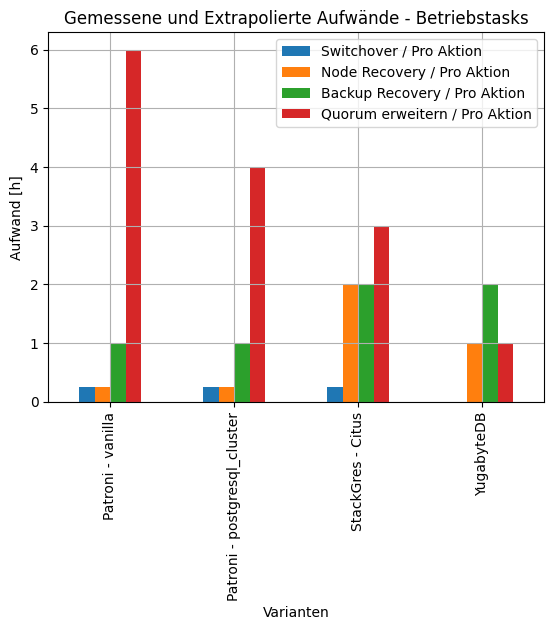
\includegraphics[width=0.75\linewidth]{source/pandas_data_chart_plotter/time_investment_action}
        \caption{Zeitaufwände pro Betriebstask}
        \label{fig:time_investment_action}
    \end{figure}
\end{flushleft}
\clearpage
\begin{flushleft}
    Daraus ergeben sich folgende gesamten Zeitaufwände, wenn sie auf 5 Jahre extrapoliert werden:
    \begin{figure}[H]
        \centering
        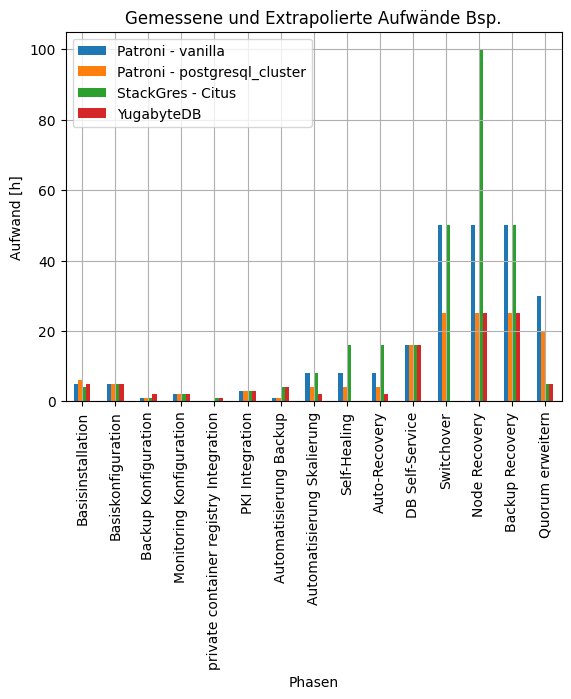
\includegraphics[width=1\linewidth]{source/pandas_data_chart_plotter/time_investment}
        \caption{Zeitaufwände}
        \label{fig:time_investment}
    \end{figure}
\end{flushleft}
\clearpage
\begin{flushleft}
    In der Summe müssen für die jeweiligen Varianten also mit folgenden Aufwänden gerechnet werden:
    \begin{figure}[H]
        \centering
        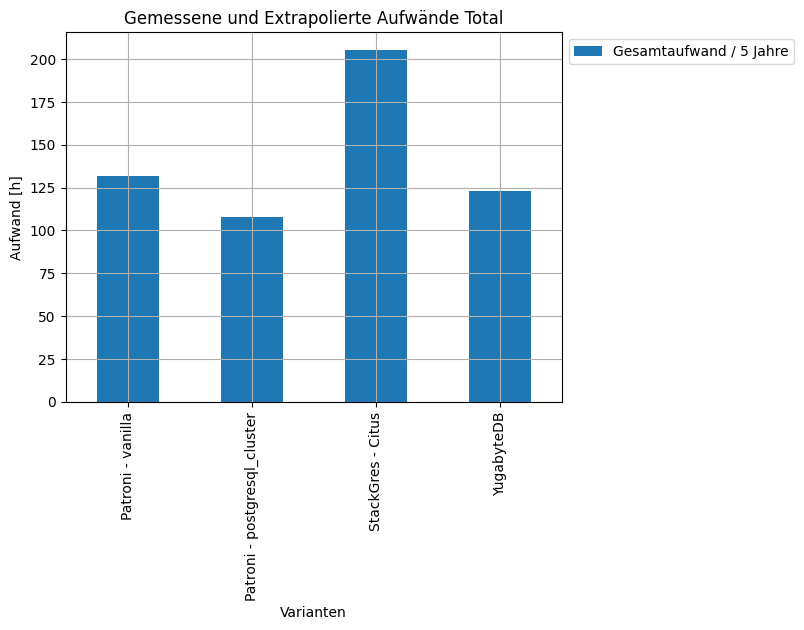
\includegraphics[width=0.65\linewidth]{source/pandas_data_chart_plotter/time_investment_summe}
        \caption{Zeitaufwände summiert}
        \label{fig:time_investment_summe}
    \end{figure}
    \paragraph{Kostenvergleiche}
    Die Kostenhochrechnung ist simpel.\\
    Da der Stundenansatz in der ICT 120 Franken pro Stunde beträgt, wurden die Zeiten einfach mit 120 multipliziert.
\end{flushleft}
\begin{flushleft}
    Für die Betriebstasks wurden daher mit folgenden Kosten gerechnet:
    \begin{figure}[H]
        \centering
        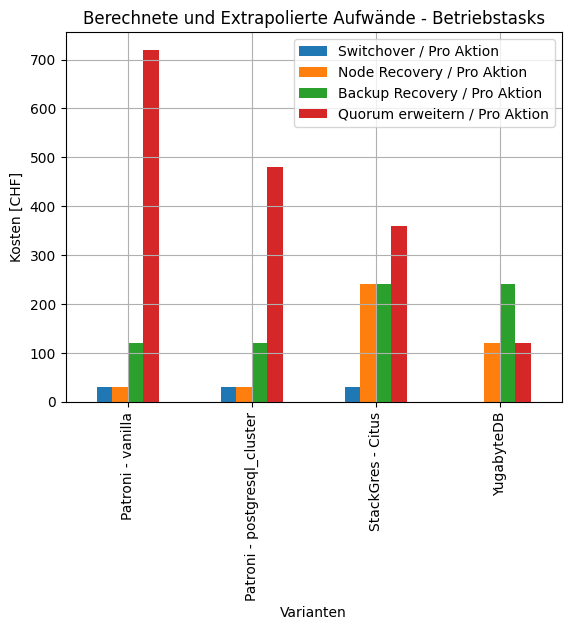
\includegraphics[width=0.65\linewidth]{source/pandas_data_chart_plotter/cost_investment_action}
        \caption{Kostenaufwände pro Betriebstask}
        \label{fig:cost_investment_action}
    \end{figure}
\end{flushleft}
\begin{flushleft}
    Anhand der Aufwände wurden die Kosten geschätzt und extrapoliert:
    %! Author = gramic
%! Date = 23.05.24

% Preamble
\begin{table}[H]
\centering
\resizebox{\columnwidth}{!}{%
\begin{tabular}{@{}llllll@{}}
\toprule
Phase                                           & Suphase                                & Patroni - vanilla & Patroni - postgresql-cluster & StackGres - Citus & YugabyteDB \\ \midrule
\multirow{4}{*}{Initialer Aufwand}              & Basisinstallation                      & 600               & 720                          & 480               & 600        \\
                                                & Basiskonfiguration                     & 600               & 600                          & 600               & 600        \\
                                                & Backup Konfiguration                   & 120               & 120                          & 120               & 240        \\
                                                & Monitoring Konfiguration               & 240               & 240                          & 240               & 240        \\
\multirow{2}{*}{Secuirty Aufwand}               & private container registry Integration & 0                 & 0                            & 120               & 120        \\
                                                & PKI Integration                        & 360               & 360                          & 360               & 360        \\
\multirow{5}{*}{Erweiterungsaufwand}            & Automatisierung Backup                 & 120               & 120                          & 480               & 480        \\
                                                & Automatisierung Skalierung             & 960               & 480                          & 960               & 240        \\
                                                & Self-Healing                           & 960               & 480                          & 1920              & 0          \\
                                                & Auto-Recovery                          & 960               & 480                          & 1920              & 240        \\
                                                & DB Self-Service                        & 1920              & 1920                         & 1920              & 1920       \\
\multirow{4}{*}{Operationsaufwand / Pro Aktion} & Switchover                             & 120               & 60                           & 120               & 0          \\
                                                & Node Recovery                          & 240               & 120                          & 480               & 120        \\
                                                & Backup Recovery                        & 240               & 120                          & 240               & 120        \\
                                                & Quorum erweitern                       & 720               & 480                          & 120               & 120        \\
\multirow{4}{*}{Operationsaufwand / 5 Jahre}    & Switchover                             & 6000              & 3000                         & 6000              & 0          \\
                                                & Node Recovery                          & 6000              & 3000                         & 12000             & 3000       \\
                                                & Backup Recovery                        & 6000              & 3000                         & 6000              & 3000       \\
                                                & Quorum erweitern                       & 3600              & 2400                         & 600               & 600        \\ \midrule
\multicolumn{2}{l}{Gesamtaufwand}                                                        & 15570             & 12810                        & 24300             & 14400      \\ \bottomrule
\end{tabular}%
}
\caption{Gemessene und extrapolierte Kosten}
\label{tab:cost_investment}
\end{table}
%    Entsprechend entstehen ist auf fünf Jahre verteilt, mit folgenden Kosten zu rechnen:
    Entsprechend ist auf fünf Jahre mit folgenden Kosten zu rechen:
    \begin{figure}[H]
        \centering
        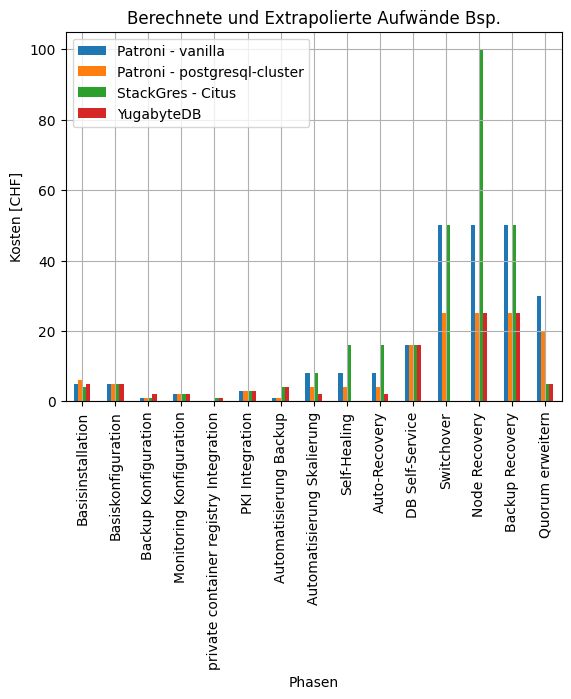
\includegraphics[width=0.75\linewidth]{source/pandas_data_chart_plotter/cost_investment}
        \caption{Kostenaufwände}
        \label{fig:cost_investment}
    \end{figure}
\end{flushleft}
\begin{flushleft}
    Die totalen geschätzten Kosten würden sich im Vergleich wie folgt entwickeln:
    \begin{figure}[H]
        \centering
        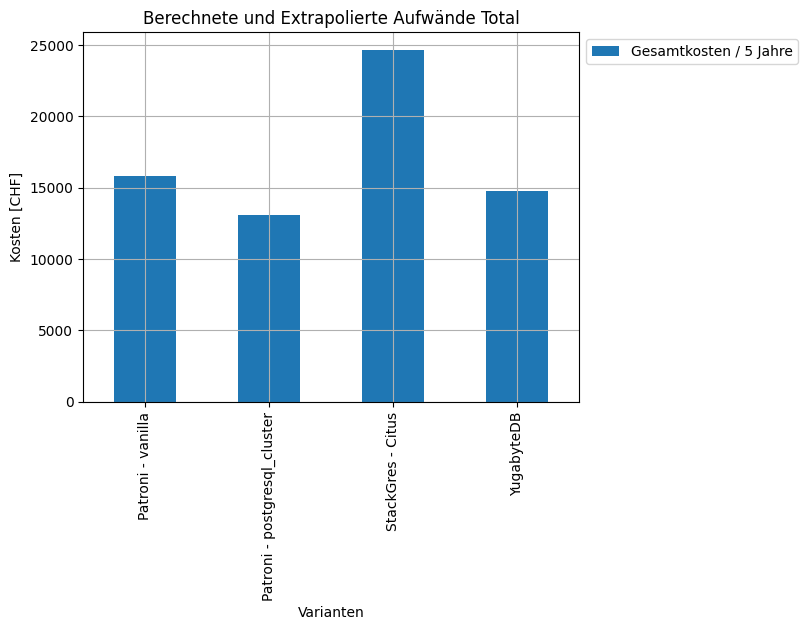
\includegraphics[width=0.75\linewidth]{source/pandas_data_chart_plotter/cost_investment_summe}
        \caption{Kostenaufwände Total}
        \label{fig:cost_investment_summe}
    \end{figure}
\end{flushleft}
%\begin{flushleft}
%    \paragraph{Schlussfolgerung}
%\end{flushleft}
